%% Description: 
%%
%%

\section {Architecture and Basic Concepts}

The PyOPC framework supports the rapid development of OPC XML-DA compliant
clients and servers and provides the following features:

\begin{description}
\item[Open source:] PyOPC and all underlying technologies are
open source projects.

\item[Multi-platform capable:] The underlying programming language of
PyOPC is Python, which is available on most platforms, such as
Microsoft Windows, Linux, Mac OS X and others. Applications built with
PyOPC can be run on all platforms with Python support. A good
introduction to the Python programming language can be found in
\cite{diveintopython} and \cite{PYTHON}.

\item[Ease of use:] Various complex functionality of the OPC XML-DA
specification is automatically handled by the PyOPC framework,
therefore the developer does not need to cope with it. Nevertheless,
the programmer may also choose to override this functionality and
thus implement it in his own way.

\item[Extensible and reusable:] Basic framework functionality
can be extended by the programmer, moreover, OPC servers built with
PyOPC can be added to the framework as a custom libraries, which can
then be reused by other applications.
\end{description}

An OPC XML-DA compliant framework needs to support several
technologies, especially building servers which process concurrent
requests and handle the SOAP and HTTP protocol. Although Python has an
extensive collection of libraries, it does not fulfill these
requirements. Therefore two additional Python frameworks are used,
which have to be available on systems that provide PyOPC based
applications. These basic technologies are illustrated in figure
\ref{technologies}.

\begin{figure}[ht]
\htmlborder{1}
\centering
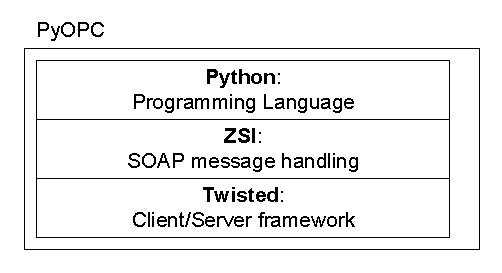
\includegraphics[scale=0.7]{graphics/technologies.eps}
\caption{Underlying Technologies of the PyOPC Framework}
\label {technologies} 
\end{figure}

\begin{description}
\item[Zolera Soap Infrastructure (ZSI):] This SOAP framework enables
parsing and serializing SOAP messages. PyOPC uses ZSI to read and
create OPC XML-DA compliant SOAP messages\footnote{This process is
hidden from developers, instead PyOPC provides abstract Python objects
for accessing underlying SOAP messages.}.

\item[Twisted:] Twisted is an asynchronous client/server framework.
It implements a variety of Internet protocols, such as HTTP and SMTP
and uses an event based mechanism to enable the development of
clients and servers which can handle concurrent requests.

In order to develop applications with Twisted, the programmer has
to lay out his program according to this event-based architecture.
Therefore building complex server applications with PyOPC require
some understanding of the basic concepts of Twisted. More information
about this framework can be found at \cite{TWISTED}.
\end{description}

\subsection {Basic PyOPC Architecture}

The PyOPC framework supports the development of OPC XML-DA client and
server applications. The OPC XML-DA standard defines the following
eight operations, which can be used to access OPC data:

\begin{description}
\item[GetStatus:] This operation is used to retrieve status information of
the OPC server.
\item[Read/Write:] These operations are used to read and write OPC
items\footnote{OPC items are basically containers which may hold a
piece of information. They resemble fieldbus data points and may
contain arbitrary data.}.
\item[Subscribe / SubscriptionPolledRequest / SubscriptionCancel:]
These operations are used to handle OPC subscriptions.
\item[Browse:] This operation is used to browse OPC items.
\item[GetProperties:] OPC items have so-called properties, which
define and describe the item. GetProperties can be used to retrieve
these OPC item properties.
\end{description}

Associated to each of these operation is a request and response SOAP
message, resulting in 16 different messages. With ZSI, these messages
can be parsed and serialized through specific Python objects,
so-called ``Typecodes''. Although accessing typecodes is far easier
than accessing the SOAP message itself, it is still a tedious
task. Therefore PyOPC hides this process from the developer by
defining various methods, which automatically handle the ZSI
typecodes. 

PyOPC introduces several classes, which are used throughout the
framework. These classes inherit from each other, forming a class
hierarchy, as illustrated in figure \ref{object_hierarchy}.

\begin{figure}[ht]
\htmlborder{1}
\centering
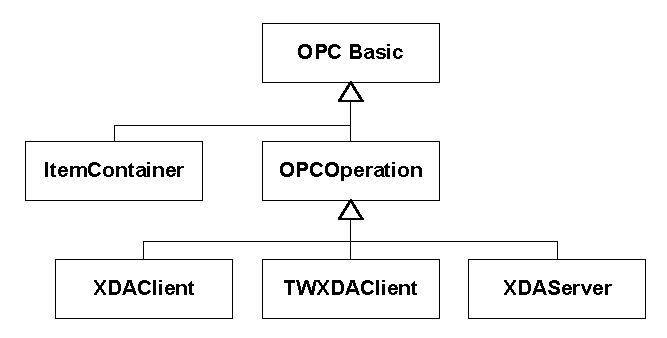
\includegraphics[scale=0.7]{graphics/object_hierarchy.eps}
\caption{Class Hierarchy of the PyOPC Framework}
\label {object_hierarchy} 
\end{figure}

The classes of this hierarchy implement the following functionality:

\begin{description}
\item[OPC Basic:] This class implements basic issues that are used by
other inheriting classes. Apart from several utility methods, the
class defines all OPC errors.
\item[OPCOperation:] The OPCOperation class handles the generation and
parsing of all OPC XML-DA SOAP messages. The class implements two read
and write methods for each operation\footnote{Every request and
response SOAP message has each a read and write method.}, which are
automatically utilized for handling ZSI typecodes.
\item[ItemContainer:] This class represents OPC items and is
described in detail below.
\item[XDAClient:] Simple OPC XML-DA clients may be built with this
class.
\item[TWXDAClient:] This class is an advanced way to build OPC XML-DA
compliant clients. The TWXDAClient class utilizes Twisted to enable
multiple, concurrent client requests.
\item[XDAServer:] The XDAServer class is the base to implement OPC
XML-DA compliant servers with the PyOPC framework.
\end{description}

\subsection {Representation of OPC XML-DA Data with Python Objects}

As already mentioned, handling SOAP messages with ZSI is not
simple. Therefore specific objects are defined by PyOPC which can be
easily accessed and represent the corresponding SOAP messages.

OPC XML-DA compliant SOAP messages contain various options which may
either concern the whole operation (global options) or may be item
specific (local options).  After closely examining these messages, it
was found that these options can be mapped to two certain Python
objects as depicted in figure \ref{message_basic}.

\begin{figure}[ht]
\htmlborder{1}
\centering
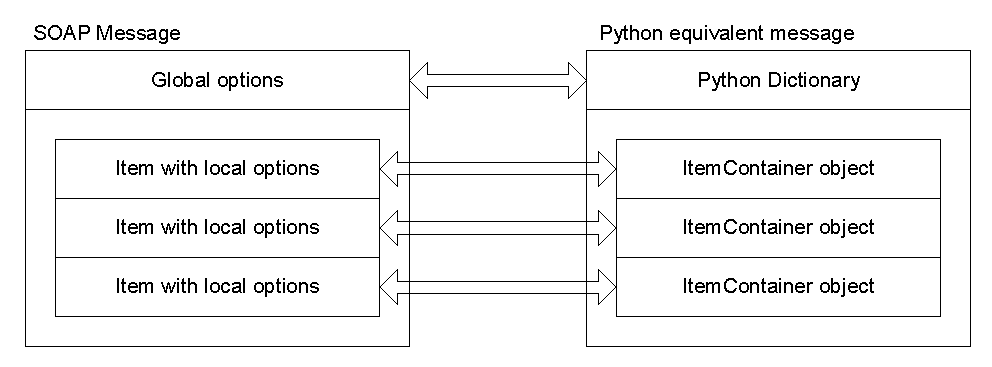
\includegraphics[scale=0.7]{graphics/message_basic.eps}
\caption{Python Objects Representing OPC XML-DA Messages}
\label {message_basic} 
\end{figure}

These two Python objects are the basic containers in the PyOPC
framework and are used to transport OPC data. Therefore they are used
as parameters for methods which represent OPC XML-DA operations.
Listing \ref{ex_message_basic} shows an example of an OPC XML-DA read
operation.

\lstset{language=C}
\begin{lstlisting}[caption={Usage of Python objects for representing
global and local options of a OPC XML-DA compliant SOAP message}
                   ,label=ex_message_basic] 
item = ItemContainer(ItemName='test_name', MaxAge=500)
item_list,global_options = xda.Read([item], ItemPath='test_path')
\end{lstlisting}

In line 1, an ItemContainer object is created, which contains the item
specific (local) options ``ItemName'' and ``MaxAge''. In line 2 the
read operation is taking place, with a list of ItemContainer objects
as the first parameter and the global option ``ItemPath'' as the
second.  The results of the read operation also consist of a list of
ItemContainer objects and a Python dictionary, containing the local
and global options.

Global and local options may sometimes be the same. In this case, the
local options override the global ones. For instance, if the option
``ItemPath'' is specified globally and locally, the local, item
specific ItemPath will have precedence.

As this mechanism is the same for all operations, it is sometimes
possible to set options that have no meaning for the current
operation. However, only relevant options will be included in the
resulting SOAP message, other options are ignored by the PyOPC
framework.  For instance, setting the option ``MaxAge'' for an OPC
Write operation has no effect at all.

There are a number of options that can be set for OPC XML-DA
operations, which can be looked up in \cite{OPCXMLDA}. These options
are case sensitive, for instance ``MaxAge'' and ``maxage'' are handled
as a different option.


\subsubsection*{Global OPC XML-DA options}

Python dictionaries are used to represent global options. As denoted
above, these dictionaries can then be used as parameters for OPC
operations.  However, often it is handy to define default global
options that are used all over the application. For instance, it may
make sense to define a server-specific default ``MaxAge'' option,
which is automatically assigned to all according SOAP messages.

Therefore PyOPC allows to specify these global options at the creation
of the client or server object, such as shown in listing \ref{ex_global}.
These global options will then be used for all operations, unless they
are overridden by global options in the method parameters.

\lstset{language=C}
\begin{lstlisting}[caption={Assigning Global Options to a PyOPC 
Client Instance}
                   ,label=ex_global]
xda = XDAClient(ReturnErrorText=False,
                ReturnItemName=True,
                ReturnDiagnosticInfo=True,
                ItemPath='')
\end{lstlisting}

The PyOPC framework always checks if global options, which are passed
as method parameters, can be applied to the current OPC operation. If
an option is unknown or misspelled, a Python {\sl TypeError} will be
raised. This way, errors due to accidental misspellings or improper
use of options are prevented.

\subsubsection*{The ItemContainer Object}

The ItemContainer object is used to store all local, item-specific OPC
XML-DA data, such as the item value and item-specific local
options. This information is stored in the object as object attributes
and may be accessed as shown in listing \ref{ex_itemcontainer}.


\lstset{language=C}
\begin{lstlisting}[caption={Accessing the PyOPC ItemContainer Object}
                   ,label=ex_itemcontainer] 
from PyOPC.OPCContainers import *
item = ItemContainer(ItemName='test_name',
                     MaxAge=500)
item.ItemName='other_name'
maxage = item.MaxAge
\end{lstlisting}

At the beginning of the example listing, the appropriate Python module
is imported that contains the ItemContainer class. In line 2, item
specific options are set at initialization time of the ItemContainer
object, while line 4 and 5 show how to directly set and retrieve
object attributes.

\cite{OPCXMLDA} defines numerous, sometimes complex local
options. Therefore errors due to misspellings can easily happen. To
prevent such errors, the ItemContainer class defines all possible
options via class attributes. In addition, an ItemContainer object
will not allow the setting of undefined object attributes. If the
developer accidentally tries to set a misspelled or unknown attribute,
the PyOPC framework raises a Python AttributeError.

\subsubsection*{Qualified Names (QNames) and Namespaces}

The OPC XML-DA specification and its associated SOAP messages
sometimes contain {\sl Qualified Names} (QNames). QNames consist of a
namespace, most often in the form of an Uniform Resource Locator (URL)
and a name. For this purpose, PyOPC defines a simple {\sl QName}
object, which is similar to a Python tuple.

Moreover PyOPC defines in the module {\sl utils} the following global
variables which may be used as the namespace part for QNames:

\begin{itemize}
\item{\sl NS\_XSD}, the namespace for XML-Schema
\item{\sl NS\_ZSI}, the ZSI namespace
\item{\sl NS\_XDA}, the namespace of the OPC XML-DA specification
\item{\sl NS\_PYO}, the PyOPC namespace
\end{itemize}

An example how to create and access such a QName object is given
in example \ref{ex_qnames}, showing the creation of a predefined 
and a custom QName in line 3 and 4 and accessing parts of the
QName in line 5:

\lstset{language=C}
\begin{lstlisting}[caption={Handling Qualified Names (QNames) with PyOPC}
                   ,label=ex_qnames] 
from PyOPC.utils import *

qn1 = QName(NS\_XSD,'string')
qn2 = QName('http://my/name/space','test123')
url, name = qn2.URI, qn2.name
\end{lstlisting}

\subsubsection*{OPC Item Properties}

Every OPC Item may have so-called {\sl properties} that contain
further information about the item. Example properties would be the
access rights or a description of the item. These OPC properties are
modeled as a specific Python object, called {\sl OPCProperty}, which
contains the following information:

\begin{description}
\item[Name:] The name uniquely identifies an OPC property. Names must
be of the type {\sl QName}.
\item[Value:] Properties most often have a value, for instance in case
of a property ``accessRights'', it stores the strings {\sl readable}
or {\sl writable}.
\item[Description:] In order to easily understand the meaning of a 
property, it can store a description.
\item[ItemPath/ItemName:] The address of the property, consisting of
the ItemPath and ItemName. 
\item[ResultID/ErrorText:] In case a property is erroneous, for
instance if it cannot be read or does not exist, the error can be
stored in a ResultID and a descriptive error text.
\end{description}

Listing \ref{ex_properties} shows in line 1 to 5 how to create and
access a PyOPC property object.

\lstset{language=C}
\begin{lstlisting}[caption={Creating and Accessing PyOPC Properties}
                   ,label=ex_properties] 
p1 = OPCProperty(Name = QName(NS_XDA,'accessRights'),
                 Value = 'readable',
                 Description = 'Access Rights')
print p1.Name, p1.Value
p1.ItemPath = 'MyPath'                 

p2 = OPCProperty(Name = 'accessRights')
print p2.Description
\end{lstlisting}

The OPC XML-DA standard specifies various common properties, which
should be preferred over custom properties, if possible. A full list
of these available properties is given in \cite{OPCXMLDA}. The alternative
are custom properties that will often be in the namespace of
PyOPC. Therefore the framework offers a simple shortcut in creating
properties: if the property name is a string instead of a QName, PyOPC
searches in a table for a matching OPC property.  If one is found, the
OPC XML-DA namespace is used, moreover the description is filled out
automatically. If the property is unknown, the PyOPC namespace will
automatically be used. This behavior is reflected in line 7 and 8 in
listing \ref{ex_properties}.

Properties will be associated with items, therefore an ItemContainer
object provides the following methods to add, delete and list
properties:

\begin{itemize}
\item{\sl addProperty(self, property) /
addProperties(self,properties)} adds one property or a list of
properties to the ItemContainer object.
\item{\sl getProperty(self, name)} retrieves a property according to
its name
\item{\sl delProperty(self, name) / popProperty (self, name)} deletes
a property. {\sl popProperty} returns the property before deletion.
\item{\sl listProperties(self)} returns a list of all item properties.
\end{itemize}


\subsubsection*{Representation of the Item Value with PyOPC Data Types}

OPC items have a {\sl value}, containing the actual information, which
corresponds to the value of a fieldbus data point. This value will be
of a certain OPC data type, such as string or integer but also more
complex types, such as an array. In order to access this information,
PyOPC has to map the OPC data type to a corresponding Python data
type, resulting in a possible data conversion. Table \ref{dataconv}
describes all possible data conversions.

\begin{table}[ht]
\htmlborder{1}
\centering
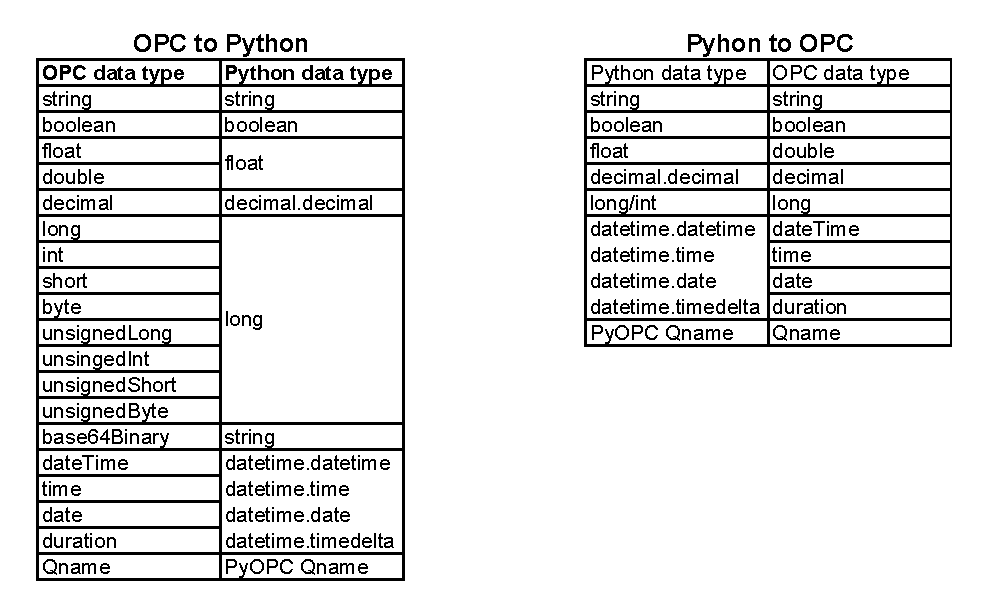
\includegraphics[scale=0.7]{graphics/dataconv.eps}
\caption{Data Conversion Between OPC XML-DA and PyOPC}
\label{dataconv} 
\end{table}

Currently, the following data types are not supported by the PyOPC
framework\footnote{The reason for these unsupported data types is that
the underlying SOAP framework, ZSI, does also not support them.}:

\begin{itemize}
\item The {\sl decimal} data type is currently not supported at all and
cannot be used.
\item The time based data types are not fully supported. Instead of
using Pythons datetime module, all data types are converted to the
Python time type. The duration type cannot be used. During conversion,
fractions of seconds and the time zone is lost.
\item The base64Binary type is mapped to a Python string. It may be
reasonable to use a corresponding Python type instead, however this is
currently not supported.
\end{itemize}

\cite{OPCXMLDA} further defines arrays, which may contain OPC data
types from the above. These arrays are directly mapped to Python
lists\footnote{OPC XML-DA further allows to nest arrays in arrays,
however this is currently not supported by PyOPC} and its elements are
converted as shown in Table 1.

\subsection{Error Handling}

OPC XML-DA describes the following two basic error types:

\begin{itemize}
\item OPC item specific, denoting that an OPC item is not
accessible or is unknown
\item OPC operation specific, identifying errors that concern the
whole operation
\end{itemize}

These two errors are handled entirely different in both OPC XML-DA and
PyOPC.

\subsubsection*{OPC Item Specific Errors}

If an OPC item cannot be read, written, is unknown or is in any other
way erroneous, the OPC server has to inform the client. These errors
do not regard the whole operation, instead the response message, which
transports the OPC items, implements the two following options that
denote the item specific error:

\begin{description}
\item[ResultID:] Item specific errors are always outlined by the
ResultID. The OPC XML-DA specification distinguishes between so-called
error and success codes, denoting if the transported item data is
valid or not. The ResultID is of the type {\sl QName} and contains a
unique ID of the error. \cite{OPCXMLDA} defines various errors, which
are in the format of {\sl E\_FAIL} or {\sl E\_ACCESS\_DENIED}.  A
complete description of these error and success codes can be found in
\cite{OPCXMLDA}.

In case the provided OPC errors do not suffice, custom errors can be
defined. PyOPC defines a few errors in its namespace, which can also
be utilized.

\item[ErrorText:] This non-mandatory option may provide descriptive
error text, which will make the reason of an error understandable to
humans.

\end{description}

Despite of an item specific error, the response message may transport
invalid item data. Therefore OPC XML-DA applications always have to
check for the ResultID, so that item specific errors are detected.

\subsubsection*{OPC Operation Specific Errors}

If the whole operation fails, for instance if the server is busy or
malfunctioning, or if the client request is badly formatted, the
server responds with a SOAP Fault message, which contains a detailed
error description.

SOAP Faults are caught by the ZSI framework. This way PyOPC can raise
an OPC specific Python error, the {\sl OPCServerError}. The
OPCServerError inherits from ZSI's {\sl Fault} error and contains the
SOAP faultcode, the faultstring and the detail. More information about
SOAP faults can be found in \cite{SOAP1} or \cite{SOAP2}.

\thispagestyle{plain}
